\documentclass[12pt]{article}

\usepackage{geometry}
\usepackage{amsmath}
\usepackage{amsfonts}
\usepackage{graphicx}

\graphicspath{ {.} }

\geometry{
    a4paper,
    total={190mm, 277mm},
    left=10mm,
    top=10mm,
}
\pagenumbering{gobble}

\begin{document}

\begin{figure}[h]
\centering
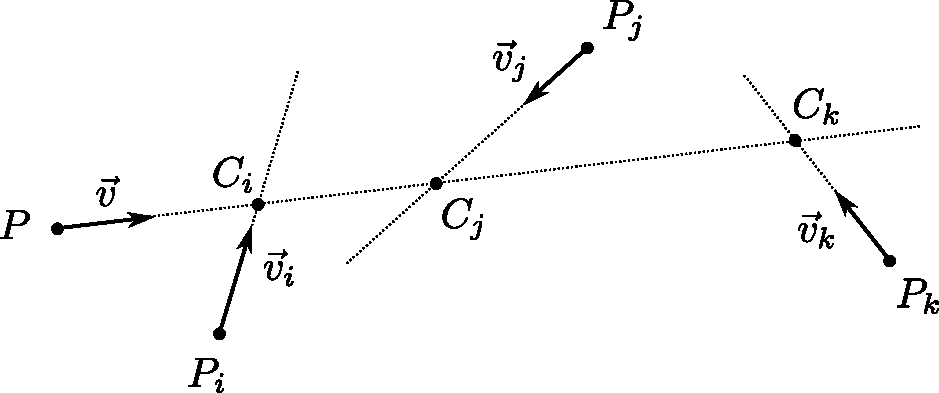
\includegraphics[scale=0.65]{particles.pdf}
\end{figure}

For all $i$, we have:
$$
C_i = P_i + t_i\vec{v}_i = P + t_i\vec{v} \;
\text{ and therefore: }
\; t_i(\vec{v}_i - \vec{v}) + P_i - P = \vec{0}
$$ \\

Hence for all $(i, j, k)$:
$$
\left\{ \begin{array}{lr}
    t_i(\vec{v}_i - \vec{v}) + P_i - P = \vec{0} & : \quad (1) \\
    t_j(\vec{v}_j - \vec{v}) + P_j - P = \vec{0} & : \quad (2) \\
    t_k(\vec{v}_k - \vec{v}) + P_k - P = \vec{0} & : \quad (3)
\end{array} \right.
$$ \\

Which gives:
$$
\left\{ \begin{array}{llr}
    (2) - (1): & (t_i - t_j) \vec{v} + t_j \vec{v}_j - t_i \vec{v}_i  + P_j - P_i = \vec{0} & : \quad (4) \\
    (3) - (1): & (t_i - t_k) \vec{v} + t_k \vec{v}_k - t_i \vec{v}_i  + P_k - P_i = \vec{0} & : \quad (5)
\end{array} \right.
$$ \\

Which in turn, with $(t_i - t_k) \times (4) - (t_i - t_j) \times (5)$, implies:
$$
t_i t_j (\vec{v}_j - \vec{v}_i) + t_j t_k (\vec{v}_k - \vec{v}_j) + t_i t_k (\vec{v}_i - \vec{v}_k) + t_i (P_j - P_k) + t_j (P_k - P_i) + t_k (P_i - P_j) = \vec{0} : \quad (6)
$$ \\

For all $i$, we note:
$$
P_i = \left[ \begin{array}{l} x_i \\ y_i \\ z_i \end{array} \right]
\text{ and }
\vec{v}_i = \left[ \begin{array}{l} v_{xi} \\ v_{yi} \\ v_{zi} \end{array} \right]
$$ \\

Furthermore, for all $(i, j)$, we note
$$
P_j - P_i =
\left[ \begin{array}{l}
x_j - x_i \\
y_j - y_i \\
z_j - z_i
\end{array} \right] =
\left[ \begin{array}{l}
\delta x_{ij} \\
\delta y_{ij} \\
\delta z_{ij}
\end{array} \right]
\text{ and }
\vec{v}_j - \vec{v}_i =
\left[ \begin{array}{l}
v_{xj} - v_{xi} \\
v_{yj} - v_{yi} \\
v_{zj} - v_{zi}
\end{array} \right] =
\left[ \begin{array}{l}
\delta v_{xij} \\
\delta v_{yij} \\
\delta v_{zij}
\end{array} \right]
$$ \\

We can now write $(6)$ as:
$$
\left\{ \begin{array}{lr}
\delta v_{xij}t_i t_j + \delta v_{xjk}t_j t_k + \delta v_{xki}t_i t_k + \delta x_{kj}t_i + \delta x_{ik}t_j + \delta x_{ji}t_k = 0 & : \quad (7) \\
\delta v_{yij}t_i t_j + \delta v_{yjk}t_j t_k + \delta v_{yki}t_i t_k + \delta y_{kj}t_i + \delta y_{ik}t_j + \delta y_{ji}t_k = 0 & : \quad (8) \\
\delta v_{zij}t_i t_j + \delta v_{zjk}t_j t_k + \delta v_{zki}t_i t_k + \delta z_{kj}t_i + \delta z_{ik}t_j + \delta z_{ji}t_k = 0 & : \quad (9)
\end{array} \right.
$$ \\

With $\delta v_{yij} \times (7) - \delta v_{xij} \times (8)$ we get:
$$
\begin{array}{l}
  \delta v_{yij}\big[\delta v_{xjk}t_j t_k + \delta v_{xki}t_i t_k + \delta x_{kj}t_i + \delta x_{ik}t_j + \delta x_{ji}t_k\big] \\
- \delta v_{xij}\big[\delta v_{yjk}t_j t_k + \delta v_{yki}t_i t_k + \delta y_{kj}t_i + \delta y_{ik}t_j + \delta y_{ji}t_k\big] \\
= (\delta v_{yij}\delta v_{xjk} - \delta v_{xij}\delta v_{yjk})t_j t_k\\
+ (\delta v_{yij}\delta v_{xki} - \delta v_{xij}\delta v_{yki})t_i t_k
\end{array}
$$ \\

\end{document}
